\chapter{Appendix}


\section{Taulas dels experiments principals} \label{s:A1}
\label{c:appendix}

En aquest apartat es recullen totes les taules corresponents als experiments realitzats durant la part pràctica del treball de recerca.

\begin{table}[p]
\centering
\resizebox{\textwidth}{!}{
\begin{tabular}{|c|c|c|}
\hline
Paràmetre & Resultats amb llum solar en mg/L & Resultats sense llum solar en mg/L \\
\hline
pH    & 6.2      & 6.2 \\
\hline
Alcalinitat total(CaCO$_3$)    & 0    & 0 \\
\hline
Carbonat     & 0      & 0 \\
\hline
Duresa (GH)   & 50          & 175  \\
\hline
Àcid cianúric    & 0     & 0 \\
\hline
Coure    & 0.2       & 0.1\\
\hline
Mercuri    & 0      & 0 \\
\hline
Clor total     & 1     & 0.5\\
\hline
 Clor lliure    & 1      & 0 \\
\hline
Brom  & 1      & 0\\
\hline
 Nitrit    & 0.5       & 0.5\\
\hline
Nitrat (NO$_3^-$)    & 10        & 25 \\
\hline
Ferro    & 0      & 0.5 \\
\hline
 Crom (VI)   & 0      & 0  \\
\hline
Plom   & 0     & 0  \\
\hline
Fluorur (F$^-$)    & 0      & 0 \\
\hline
\end{tabular}%
}
\caption{Resultats del primer experiment}
\label{tab:comparacio_dades}
\end{table}

\begin{table}[p]
\centering
\resizebox{\textwidth}{!}{
\begin{tabular}{|l|c|c|c|p{4.4cm}|}
\hline
\textbf{Paràmetre} & \textbf{Valor experimental} & \textbf{Valor oficial} & \textbf{Unitats} & \textbf{Comentari} \\
\hline \hline
pH & 6,2 & 7.2-8.3 & unitats pH & Inferior al valor oficial; aigua més àcida. \\
\hline
Alcalinitat total & 0 & 158-210 & mg CaCO$_3$/L & Valor experimental probablement incorrecte. \\
\hline
Carbonats & 0 & --- & mg /L & Informació no proporcionada. \\
\hline
Duresa total & 50 & 222-309 & mg GH /L & Molt inferior al valor oficial. \\
\hline
Nitrat & 10 & 5.2-11.1 & mg NO$_3^-$ /L & Lleugerament superior; dins de marges acceptables. \\
\hline
Nitrit & 0.5 & ---& mg /L & Informació no proporcionada. \\
\hline
Clor total & 1 & --- & mg/L & Valor comú en aigües potables. \\
\hline
Clor lliure & 1 & --- & mg/L & Idèntic al valor anterior. \\
\hline
Ferro & 0 & --- & mg/L & No detectat; valor desitjable. \\
\hline
Fluorur & 0 & $<$0,2 & mg F$^-$ /L & Coincideix amb el límit inferior. \\
\hline
Crom (VI) & 0 & --- & mg/L & No present, tal com és recomanable. \\
\hline
Plom & 0 & --- & mg/L & Absent, com hauria de ser. \\
\hline
Àcid cianúric & 0 & --- & mg/L & No rellevant en aigua potable. \\
\hline
Coure & 0,2 & --- & mg/L & Informació no detectada en aquest cas. \\
\hline
Brom & 1 & --- & mg/L & No habitual en aigua potable. \\
\hline
Mercuri & 0 & --- & mg/L & No present; correcte. \\
\hline
\end{tabular}%
}
\caption{Comparació entre els valors experimentals i els oficial (amb exposició solar)}
\label{tab:comparacio_aigua_amb_sol}
\end{table}

\begin{table}[p]
\centering
\resizebox{\textwidth}{!}{%
\begin{tabular}{|l|c|c|c|p{4.2cm}|}
\hline
\textbf{Paràmetre} & \textbf{Valor experimental} & \textbf{Valor oficial} & \textbf{Unitats} & \textbf{Comentari} \\
\hline \hline
pH & 6,2 & 7.2-8.3 & unitats pH & Inferior al valor oficial; aigua més àcida. \\
\hline
Alcalinitat total & 0 & 158-210 & mg CaCO$_3$/L & Valor experimental probablement incorrecte. \\
\hline
Carbonats & 0 & --- & mg /L & Informació no proporcionada. \\
\hline
Duresa total & 175 & 222-309 & mg GH/L & Millor aproximació al valor real que abans. \\
\hline
Nitrat & 25 & 5.2-11.1 & mg NO$_3^-$ /L & Molt lluny al valor oficial. \\
\hline
Nitrit & 0.5 & ---& mg /L & Informació no proporcionada. \\
\hline
Clor total & 0,5 & --- & mg/L & Ligerament inferior a la prova amb sol. \\
\hline
Clor lliure & 0 & --- & mg/L & Idèntic al total; valor típic. \\
\hline
Ferro & 0.5 & --- & mg/L & Ligerament superior al valor amb sol; no hauria de tenir. \\
\hline
Fluorur & 0 & $<$0,2 & mg F$^-$ /L & Coincideix amb el valor esperat. \\
\hline
Crom (VI) & 0 & --- & mg/L & No present. \\
\hline
Plom & 0 & --- & mg/L & No detectat; adequat. \\
\hline
Àcid cianúric & 0 & --- & mg/L & No rellevant; igual que en la prova anterior. \\
\hline
Coure & 0,1 & --- & mg/L & Informació no detectada en aquest cas. \\
\hline
Brom & 0 & --- & mg/L & No detectat en aquest cas. \\
\hline
Mercuri & 0 & --- & mg/L & No detectat; correcte. \\
\hline
\end{tabular}%
}
\caption{Comparació entre els valors experimentals i els oficials (sense exposició solar)}
\label{tab:comparacio_aigua_sense_sol}
\end{table}

\begin{table}[H]
\centering
\resizebox{\textwidth}{!}{
\begin{tabular}{|c|c|c|}
\hline
Paràmetre & Resultats sense llum en mg/L & Resultats amb llum en mg/L \\
\hline
pH    & 7.8      & 7.6 \\
\hline
Alcalinitat total(CaCO$_3$)    & 40    & 120 \\
\hline
Carbonat     & 0     & 80 \\
\hline
Duresa (GH)   & 200          & 425  \\
\hline
Àcid cianúric    & 0     & 0 \\
\hline
Coure    & 0.2       & 0.2\\
\hline
Mercuri    & 0      & 0 \\
\hline
Clor total     & 0     & 0\\
\hline
 Clor lliure    & 0      & 0 \\
\hline
Brom  & 0      & 0\\
\hline
 Nitrit    & 0       & 0\\
\hline
Nitrat (NO$_3^-$)    & 0        & 0 \\
\hline
Ferro    & 0      & 0 \\
\hline
 Crom (VI)   & 0      & 0  \\
\hline
Plom   & 0     & 0  \\
\hline
Fluorur (F$^-$)    & 0      & 0 \\
\hline
\end{tabular}%
}
\caption{Resultats del experiment 2}

\label{tab:comparacio_dades2}
\end{table}

\begin{table}[H]
\centering
\resizebox{\textwidth}{!}{%
\begin{tabular}{|l|c|c|c|p{4.2cm}|}
\hline
\textbf{Paràmetre} & \textbf{Valor experimental} & \textbf{Valor oficial} & \textbf{Unitats} & \textbf{Comentari} \\
\hline \hline
pH & 7.8 & 7,3-8.3 & unitats pH & Dins dels valors minim-màxim.. \\
\hline
Alcalinitat total & 40 & 65.3-217 & mg CaCO$_3$/L & Valor experimental probablement incorrecte. \\
\hline
Carbonats & 0 & --- & mg /L & Informació no proporcionada. \\
\hline
Duresa total & 200 & 75.3-424 & mg GH/L & Millor aproximació al valor real que l'anterior experiment; dins dels valors minim-màxim. \\
\hline
Nitrat & 0 & $<$1-10.2 & mg NO$_3^-$ /L & Dins dels valors oficial. \\
\hline
Nitrit & 0 & ---& mg /L & Informació no proporcionada. \\
\hline
Clor total & 0 & --- & mg/L & Valor típic \\
\hline
Clor lliure & 0 & --- & mg/L & Idèntic al total; valor típic. \\
\hline
Ferro & 0 & --- & mg/L & Adequat; no hauria de tenir. \\
\hline
Fluorur & 0 & $<$0,2 & mg F$^-$ /L & Coincideix amb el valor esperat. \\
\hline
Crom (VI) & 0 & --- & mg/L & No present. \\
\hline
Plom & 0 & --- & mg/L & No detectat; adequat. \\
\hline
Àcid cianúric & 0 & --- & mg/L & No rellevant; igual que en l'experiment anterior. \\
\hline
Coure & 0.2 & --- & mg/L & Informació no detectada en aquest cas. \\
\hline
Brom & 0 & --- & mg/L & No detectat en aquest cas. \\
\hline
Mercuri & 0 & --- & mg/L & No detectat; correcte. \\
\hline
\end{tabular}%
}
\caption{Comparació entre els valors experimentals i els oficials de l'aigua del bar (sense exposició a cap font de llum}
\label{tab:comparacio_aigua_sense_llum}
\end{table}

\begin{table}[H]
\centering
\resizebox{\textwidth}{!}{%
\begin{tabular}{|l|c|c|c|p{4.2cm}|}
\hline
\textbf{Paràmetre} & \textbf{Valor experimental} & \textbf{Valor oficial} & \textbf{Unitats} & \textbf{Comentari} \\
\hline \hline
pH & 7.6 & 7,3-8.3 & unitats pH & Dins dels valors minim-màxim; com l'anterior cas. \\
\hline
Alcalinitat total & 120 & 65.3-217 & mg CaCO$_3$/L & Valor experimental dins dels limits. \\
\hline
Carbonats & 80 & --- & mg /L & Informació no proporcionada. \\
\hline
Duresa total & 425 & 75.3-424 & mg GH/L & Millor aproximació al valor real que abans, però no està dins dels valors minim-màxim; pot ser un petit error de extraccio de dades. \\
\hline
Nitrat & 0 & $<$1-10.2 & mg NO$_3^-$ /L & Dins dels valors oficial; com l'anterior cas. \\
\hline
Nitrit & 0 & ---& mg /L & Informació no proporcionada. \\
\hline
Clor total & 0 & --- & mg/L & Valor típic \\
\hline
Clor lliure   & 0 & --- & mg/L & Idèntic al total; valor típic. \\
\hline
Ferro & 0 & --- & mg/L & Adequat; no hauria de tenir. \\
\hline
Fluorur & 0 & $<$0,2 & mg F$^-$ /L & Coincideix amb el valor esperat; com l'anterior cas. \\
\hline
Crom (VI) & 0 & --- & mg/L & No present. \\
\hline
Plom & 0 & --- & mg/L & No detectat; adequat. \\
\hline
Àcid cianúric & 0 & --- & mg/L & No rellevant; igual que en l'experiment anterior. \\
\hline
Coure & 0.2 & --- & mg/L & Informació no detectada en aquest cas. \\
\hline
Brom & 0 & --- & mg/L & No detectat en aquest cas. \\
\hline
Mercuri & 0 & --- & mg/L & No detectat; correcte. \\
\hline
\end{tabular}%
}
\caption{Comparació entre els valors experimentals i els oficials de l'aigua del bar (amb exposició a gran cuantitat de llum}
\label{tab:comparacio_aigua_amb_llum}
\end{table}

\begin{figure}[H]
\centering
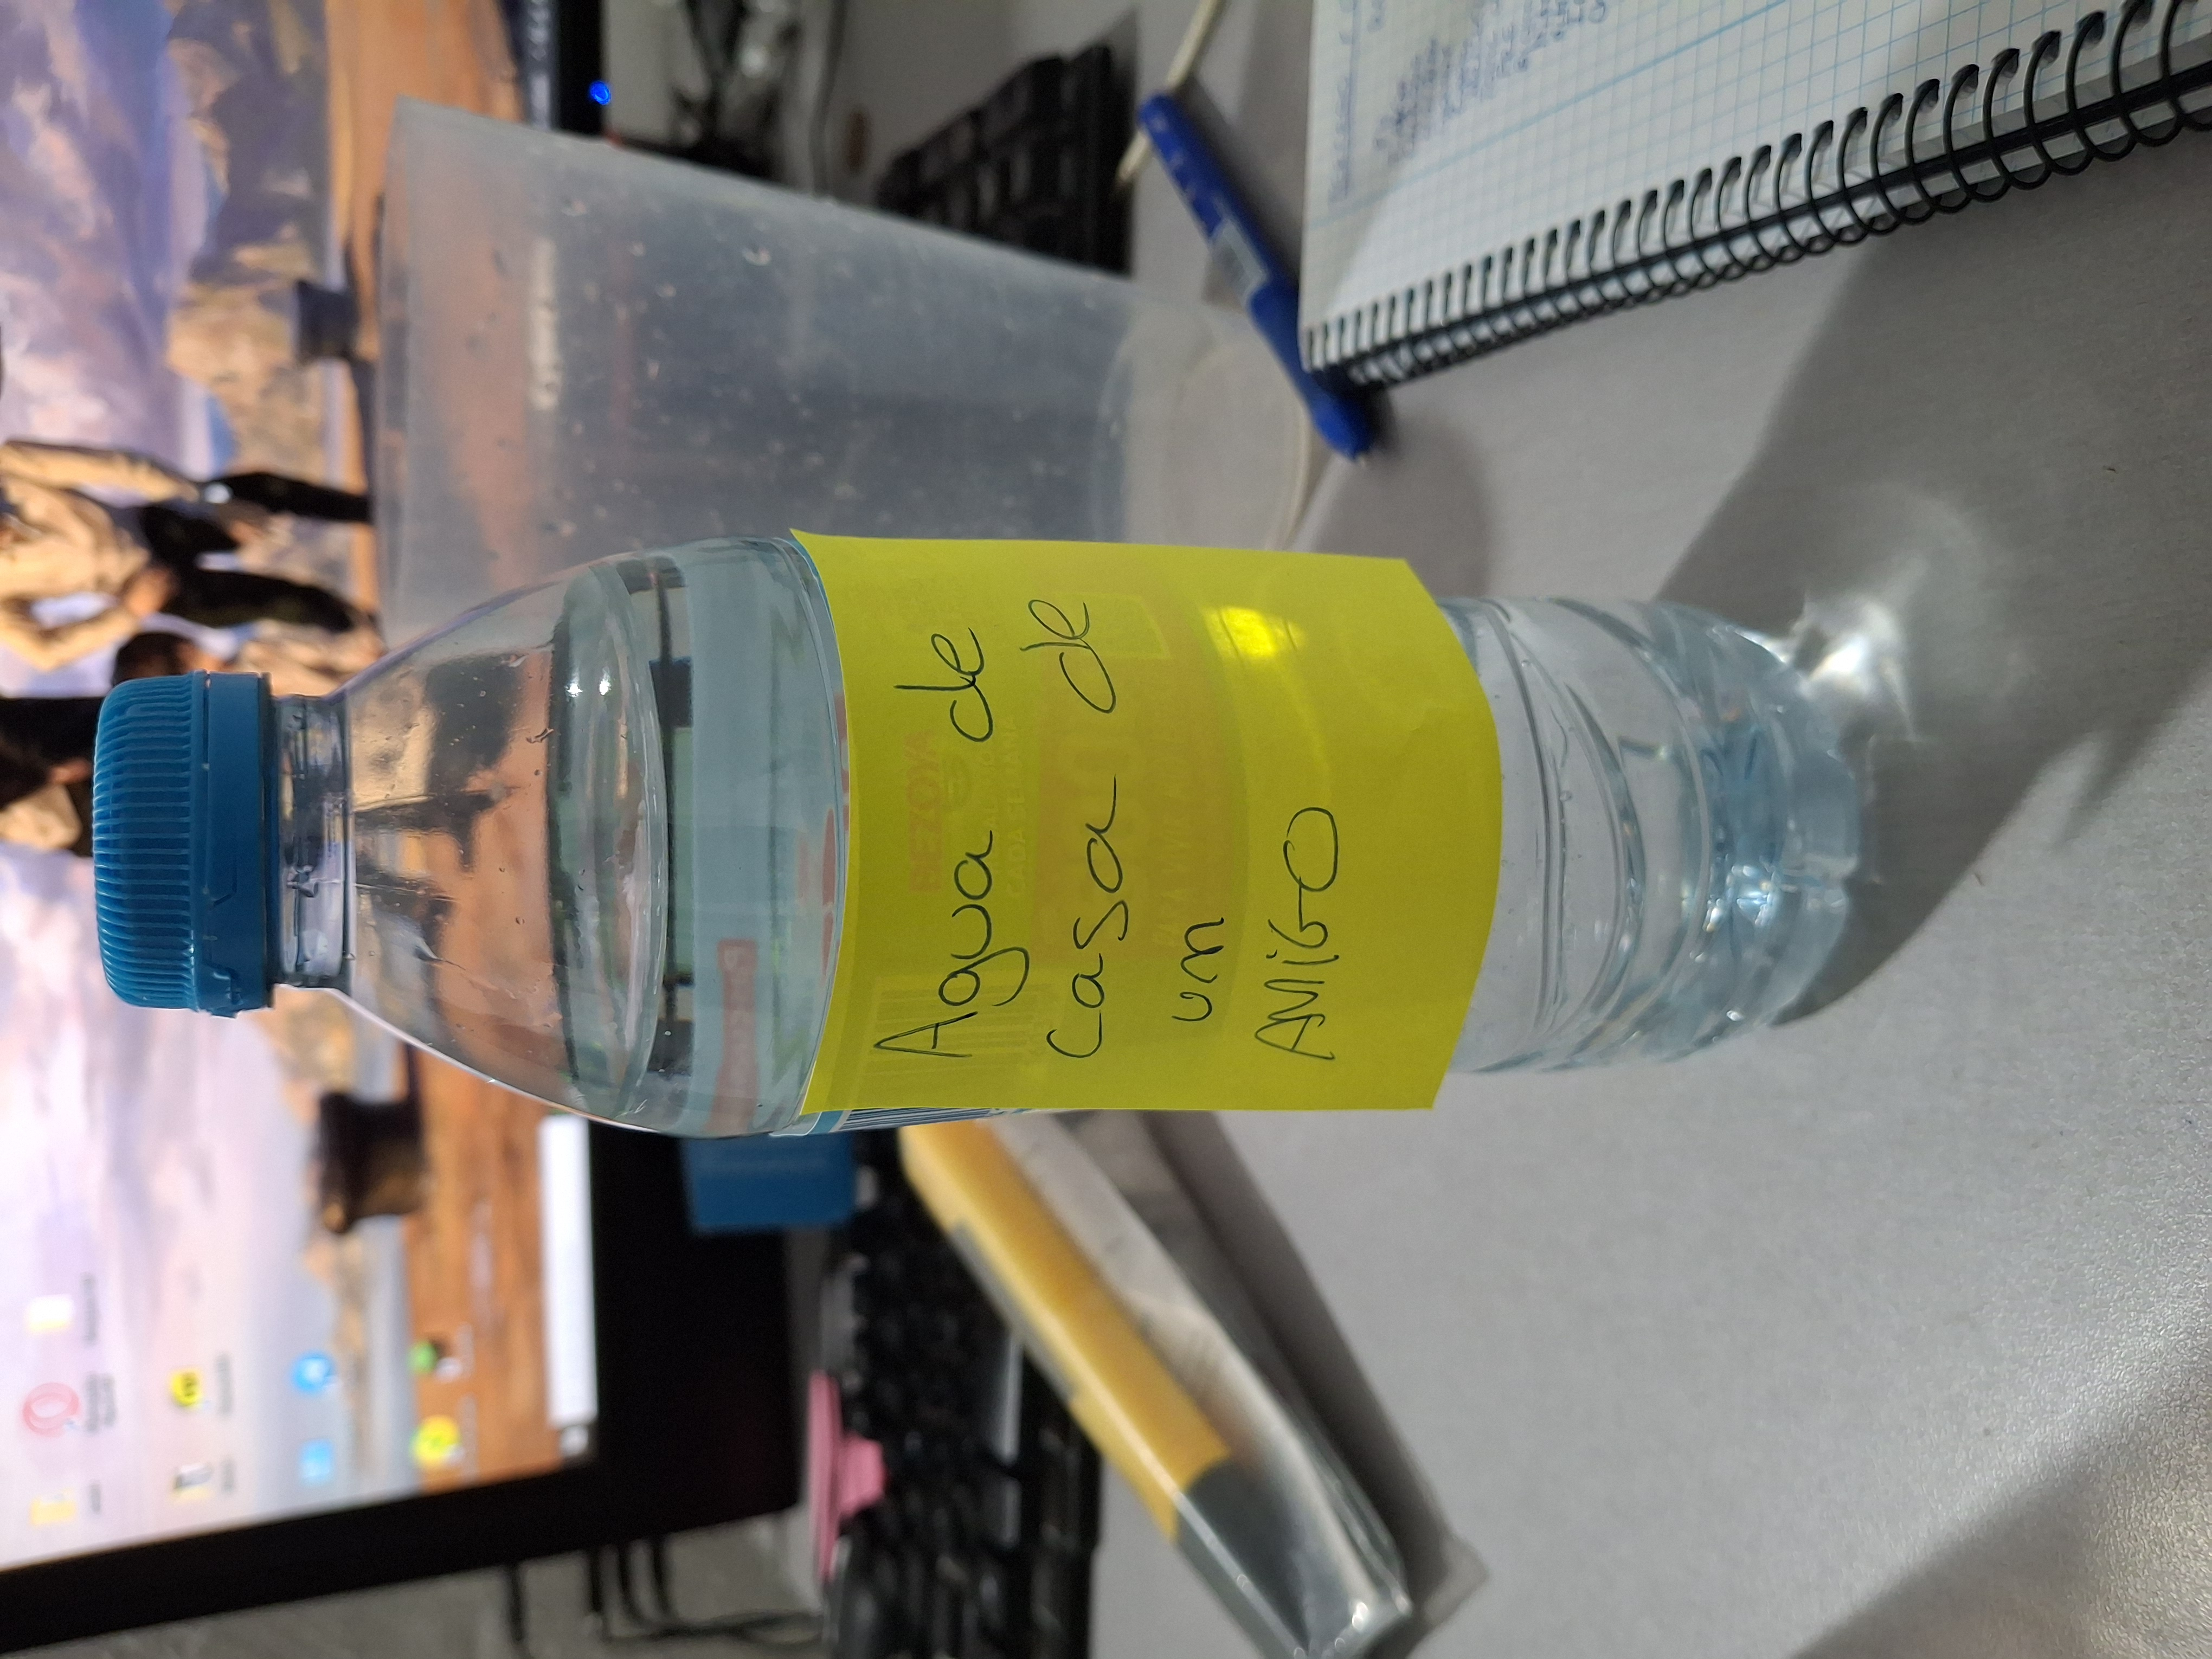
\includegraphics[width=0.5\textwidth, angle=270]{./Figures/ex3.png}
\caption{Mostra número 3}
\label{fig:Mostra3}
\end{figure}
Després de fer les proves amb les tires reactives, aquests en van ser els resultats:
\begin{table}[H]
\centering
\resizebox{\textwidth}{!}{%
\begin{tabular}{|l|c|c|c|p{4.2cm}|}
\hline
\textbf{Paràmetre} & \textbf{Tira amb durada 5 segons} & \textbf{Tira amb durada 120 segonsl} & \textbf{Unitats} & \textbf{Comentari} \\
\hline \hline
pH & 8.4 & 8.4 & unitats pH & No hi ha difèrencia en cap cas. \\
\hline
Alcalinitat total & 180 & 240 & mg CaCO$_3$/L & Difèrencia bastant elevada. \\
\hline
Carbonats & 180 & 240 & mg/L & Difèrencia bastant elevada. \\
\hline
Duresa total & 335 & 425 & mg GH/L & Difèrencia bastant elevada. . \\
\hline
Nitrat & 10 & 25 & mg NO$_3^-$ /L & Difèrencia bastant elevada. \\
\hline
Nitrit & 0 & 0 & mg /L & Cap difèrencia. \\
\hline
Clor total & 0 & 0 & mg/L & Cap difèrencia. \\
\hline
Clor lliure & 0 & 0 & mg/L & Cap difèrencia. \\
\hline
Ferro & 0 & 0 & mg/L & Cap difèrencia. \\
\hline
Fluorur & 0 & 0 & mg F$^-$ /L & Cap difèrencia. \\
\hline
Crom (VI) & 0 & 0 & mg/L & Cap difèrencia. \\
\hline
Plom & 0 & 0 & mg/L & Cap difèrencia. \\
\hline
Àcid cianúric & 0 & 0 & mg/L & Cap difèrencia. \\
\hline
Coure & 0.2 & 0.5 & mg/L & Difèrencia de 0,3 mg/L. \\
\hline
Brom & 0 & 0 & mg/L & Cap difèrencia. \\
\hline
Mercuri & 0 & 0 & mg/L & Cap difèrencia.. \\
\hline
\end{tabular}%
}
\caption{Comparació entre els valors experimentals a l'experiment 3}
\label{tab:comparacio_dades_3}
\end{table}

\begin{table}[H]
\centering
\resizebox{\textwidth}{!}{%
\begin{tabular}{|l|c|c|c|p{4.2cm}|}
\hline
\textbf{Paràmetre} & \textbf{Valor experimental} & \textbf{Valor oficial} & \textbf{Unitats} & \textbf{Comentari} \\
\hline \hline
pH & 8.4 & 7,3-8.3 & unitats pH & Supera per poc al valor màxim. \\
\hline
Alcalinitat total & 180 & 65.3-217 & mg CaCO$_3$/L & Valor experimental dins dels limits. \\
\hline
Carbonats & 180 & --- & mg /L & Informació no proporcionada. \\
\hline
Duresa total & 335 & 75.3-424 & mg GH/L & Valor experimental dins dels limits. \\
\hline
Nitrat & 10 & $<$1-10.2 & mg NO$_3^-$ /L & Valor experimental dins dels limits. \\
\hline
Nitrit & 0 & ---& mg /L & Informació no proporcionada. \\
\hline
Clor total & 0 & --- & mg/L & Valor típic \\
\hline
Clor lliure & 0 & --- & mg/L & Idèntic al total; valor típic. \\
\hline
Ferro & 0 & --- & mg/L & Adequat; no hauria de tenir. \\
\hline
Fluorur & 0 & $<$0,2 & mg F$^-$ /L & Coincideix amb el valor esperat. \\
\hline
Crom (VI) & 0 & --- & mg/L & No present. \\
\hline
Plom & 0 & --- & mg/L & No detectat; adequat. \\
\hline
Àcid cianúric & 0 & --- & mg/L & No rellevant; igual que en els experiments anteriors. \\
\hline
Coure & 0.2 & --- & mg/L & Informació no detectada en aquest cas. \\
\hline
Brom & 0 & --- & mg/L & No detectat en aquest cas. \\
\hline
Mercuri & 0 & --- & mg/L & No detectat; correcte. \\
\hline
\end{tabular}%
}
\caption{Comparació entre els valors experimentals i els oficials, tira anb durada 5 segons}
\label{tab:comparacio_aigua_5s}
\end{table}

\begin{table}[H]
\centering
\resizebox{\textwidth}{!}{%
\begin{tabular}{|l|c|c|c|p{4.2cm}|}
\hline
\textbf{Paràmetre} & \textbf{Valor experimental} & \textbf{Valor oficial} & \textbf{Unitats} & \textbf{Comentari} \\
\hline \hline
pH & 8.4 & 7,3-8.3 & unitats pH & Supera per poc al valor màxim; com abans. \\
\hline
Alcalinitat total & 240 & 65.3-217 & mg CaCO$_3$/L & Valor experimental lluny dels limits. \\
\hline
Carbonats & 240 & --- & mg /L & Informació no proporcionada. \\
\hline
Duresa total & 425 & 75.3-424 & mg GH/L & Valor experimental fora dels limits per 1 mg/L; ppot ser un error visual de part meva. \\
\hline
Nitrat & 25 & $<$1-10.2 & mg NO$_3^-$ /L & Valor experimental lluny dels limits. \\
\hline
Nitrit & 0 & ---& mg /L & Informació no proporcionada. \\
\hline
Clor total & 0 & --- & mg/L & Valor típic \\
\hline
Clor lliure & 0 & --- & mg/L & Idèntic al total; valor típic. \\
\hline
Ferro & 0 & --- & mg/L & Adequat; no hauria de tenir. \\
\hline
Fluorur & 0 & $<$0,2 & mg F$^-$ /L & Coincideix amb el valor esperat. \\
\hline
Crom (VI) & 0 & --- & mg/L & No present. \\
\hline
Plom & 0 & --- & mg/L & No detectat; adequat. \\
\hline
Àcid cianúric & 0 & --- & mg/L & No rellevant; igual que en els experiments anteriors. \\
\hline
Coure & 0.5 & --- & mg/L & Informació no detectada en aquest cas. \\
\hline
Brom & 0 & --- & mg/L & No detectat en aquest cas. \\
\hline
Mercuri & 0 & --- & mg/L & No detectat; correcte. \\
\hline
\end{tabular}%
}
\caption{Comparació entre els valors experimentals i els oficials, tira anb durada 120 segons}
\label{tab:comparacio_aigua_120s}
\end{table}

\section{Validació de la guia manual amb experiments} \label{s:A2}

Per tal de comprovar la fiabilitat i la utilitat de la guia que he elaborat sobre l’ús de les tires reactives, vaig decidir realitzar un conjunt de cinc experiments addicionals. En cadascun d’ells vaig aplicar de manera estricta les recomanacions i passos descrits a la guia, amb l’objectiu de veure si realment els resultats experimentals es mantenien dins dels marges oficials o, almenys, si mostraven una coherència clara.

Els experiments es van dur a terme en condicions diverses: lectures ràpides (5 segons), lectures amb temps més prolongat (fins a 2 minuts), i també modificant factors com la il·luminació (llum natural, llum artificial intensa i condicions òptimes). Gràcies a això, vaig poder avaluar la sensibilitat dels resultats a aquestes variables i contrastar fins a quin punt la guia ajuda a reduir errors en la presa de mesures.

A continuació es presenten les cinc taules comparatives corresponents a aquests experiments. En cadascuna d’elles es mostren, per a cada paràmetre, el valor experimental obtingut, el valor oficial de referència i un comentari interpretatiu. D’aquesta manera, les taules donen suport a la validesa de la guia com a eina per obtenir mesures més consistents i fiables amb tires reactives.


\begin{table}[H]
\centering
\resizebox{\textwidth}{!}{%
\begin{tabular}{|l|c|c|c|p{4.2cm}|}
\hline
\textbf{Paràmetre} & \textbf{Valor experimental} & \textbf{Valor oficial} & \textbf{Unitats} & \textbf{Comentari} \\
\hline \hline
pH & 7.8 & 7,3-8.3 & unitats pH & Lleugerament superior però dins dels marges oficials. \\
\hline
Alcalinitat total & 140 & 65.3-217 & mg CaCO$_3$/L & Valor adequat i ben dins del rang. \\
\hline
Carbonats & 95 & --- & mg/L & Informació no proporcionada. \\
\hline
Duresa total & 390 & 75.3-424 & mg GH/L & Aproximació correcta; dins del límit superior. \\
\hline
Nitrat & 3 & $<$1-10.2 & mg NO$_3^-$ /L & Dins del rang oficial. \\
\hline
Nitrit & 0 & --- & mg/L & Informació no proporcionada. \\
\hline
Clor total & 0.1 & --- & mg/L & Valor típic, baixa concentració. \\
\hline
Clor lliure & 0.1 & --- & mg/L & Idèntic al total. \\
\hline
Ferro & 0 & --- & mg/L & No detectat. \\
\hline
Fluorur & 0 & $<$0,2 & mg F$^-$ /L & Coincideix amb el límit. \\
\hline
Crom (VI) & 0 & --- & mg/L & No present. \\
\hline
Plom & 0 & --- & mg/L & Correcte. \\
\hline
Àcid cianúric & 0 & --- & mg/L & No rellevant. \\
\hline
Coure & 0.1 & --- & mg/L & Detectat en quantitat mínima. \\
\hline
Brom & 0 & --- & mg/L & No detectat. \\
\hline
Mercuri & 0 & --- & mg/L & Correcte. \\
\hline
\end{tabular}%
}
\caption{Experiment 1 seguint la guia manual (lectura ràpida a 5 segons)}
\label{tab:comparacio_exp1}
\end{table}


\begin{table}[H]
\centering
\resizebox{\textwidth}{!}{%
\begin{tabular}{|l|c|c|c|p{4.2cm}|}
\hline
\textbf{Paràmetre} & \textbf{Valor experimental} & \textbf{Valor oficial} & \textbf{Unitats} & \textbf{Comentari} \\
\hline \hline
pH & 7.4 & 7,3-8.3 & unitats pH & Dins del rang i força ajustat al valor real. \\
\hline
Alcalinitat total & 110 & 65.3-217 & mg CaCO$_3$/L & Correcte; dins dels límits. \\
\hline
Carbonats & 70 & --- & mg/L & No proporcionat. \\
\hline
Duresa total & 405 & 75.3-424 & mg GH/L & Molt proper al valor màxim oficial. \\
\hline
Nitrat & 6 & $<$1-10.2 & mg NO$_3^-$ /L & Correcte, dins del rang. \\
\hline
Nitrit & 0 & --- & mg/L & Informació no proporcionada. \\
\hline
Clor total & 0.2 & --- & mg/L & Liger augment respecte altres proves. \\
\hline
Clor lliure & 0.2 & --- & mg/L & Idèntic al total. \\
\hline
Ferro & 0 & --- & mg/L & No detectat. \\
\hline
Fluorur & 0.1 & $<$0,2 & mg F$^-$ /L & Coincideix amb el valor oficial. \\
\hline
Crom (VI) & 0 & --- & mg/L & No present. \\
\hline
Plom & 0 & --- & mg/L & Correcte. \\
\hline
Àcid cianúric & 0 & --- & mg/L & No rellevant. \\
\hline
Coure & 0.3 & --- & mg/L & Valor lleugerament superior; no crític. \\
\hline
Brom & 0 & --- & mg/L & No detectat. \\
\hline
Mercuri & 0 & --- & mg/L & Correcte. \\
\hline
\end{tabular}%
}
\caption{Experiment 2 seguint la guia manual (lectura amb llum artificial intensa)}
\label{tab:comparacio_exp2}
\end{table}


\begin{table}[H]
\centering
\resizebox{\textwidth}{!}{%
\begin{tabular}{|l|c|c|c|p{4.2cm}|}
\hline
\textbf{Paràmetre} & \textbf{Valor experimental} & \textbf{Valor oficial} & \textbf{Unitats} & \textbf{Comentari} \\
\hline \hline
pH & 8.1 & 7,3-8.3 & unitats pH & Força proper al límit superior, però dins del rang. \\
\hline
Alcalinitat total & 150 & 65.3-217 & mg CaCO$_3$/L & Valor adequat. \\
\hline
Carbonats & 100 & --- & mg/L & Informació no proporcionada. \\
\hline
Duresa total & 360 & 75.3-424 & mg GH/L & Dins del rang, valor mitjà. \\
\hline
Nitrat & 8 & $<$1-10.2 & mg NO$_3^-$ /L & Correcte, prop del límit superior. \\
\hline
Nitrit & 0 & --- & mg/L & Informació no proporcionada. \\
\hline
Clor total & 0 & --- & mg/L & No detectat. \\
\hline
Clor lliure & 0 & --- & mg/L & Idèntic al total. \\
\hline
Ferro & 0.1 & --- & mg/L & Lleugera presència, no preocupant. \\
\hline
Fluorur & 0 & $<$0,2 & mg F$^-$ /L & Correcte. \\
\hline
Crom (VI) & 0 & --- & mg/L & No present. \\
\hline
Plom & 0 & --- & mg/L & Correcte. \\
\hline
Àcid cianúric & 0 & --- & mg/L & No rellevant. \\
\hline
Coure & 0.2 & --- & mg/L & Present en mínima quantitat. \\
\hline
Brom & 0 & --- & mg/L & No detectat. \\
\hline
Mercuri & 0 & --- & mg/L & Correcte. \\
\hline
\end{tabular}%
}
\caption{Experiment 3 seguint la guia manual (lectura després de 30 segons)}
\label{tab:comparacio_exp3}
\end{table}


\begin{table}[H]
\centering
\resizebox{\textwidth}{!}{%
\begin{tabular}{|l|c|c|c|p{4.2cm}|}
\hline
\textbf{Paràmetre} & \textbf{Valor experimental} & \textbf{Valor oficial} & \textbf{Unitats} & \textbf{Comentari} \\
\hline \hline
pH & 7.2 & 7,3-8.3 & unitats pH & Lleugerament inferior al mínim oficial. \\
\hline
Alcalinitat total & 90 & 65.3-217 & mg CaCO$_3$/L & Correcte, dins del rang. \\
\hline
Carbonats & 65 & --- & mg/L & Informació no proporcionada. \\
\hline
Duresa total & 410 & 75.3-424 & mg GH/L & Força proper al màxim. \\
\hline
Nitrat & 2 & $<$1-10.2 & mg NO$_3^-$ /L & Dins dels marges oficials. \\
\hline
Nitrit & 0 & --- & mg/L & Informació no proporcionada. \\
\hline
Clor total & 0.3 & --- & mg/L & Valor una mica més alt que la resta. \\
\hline
Clor lliure & 0.3 & --- & mg/L & Idèntic al total. \\
\hline
Ferro & 0 & --- & mg/L & Correcte. \\
\hline
Fluorur & 0.1 & $<$0,2 & mg F$^-$ /L & Correcte. \\
\hline
Crom (VI) & 0 & --- & mg/L & No detectat. \\
\hline
Plom & 0 & --- & mg/L & Correcte. \\
\hline
Àcid cianúric & 0 & --- & mg/L & No rellevant. \\
\hline
Coure & 0.4 & --- & mg/L & Una mica elevat en comparació amb altres proves. \\
\hline
Brom & 0 & --- & mg/L & No detectat. \\
\hline
Mercuri & 0 & --- & mg/L & Correcte. \\
\hline
\end{tabular}%
}
\caption{Experiment 4 seguint la guia manual (lectura després de 2 minuts)}
\label{tab:comparacio_exp4}
\end{table}


\begin{table}[H]
\centering
\resizebox{\textwidth}{!}{%
\begin{tabular}{|l|c|c|c|p{4.2cm}|}
\hline
\textbf{Paràmetre} & \textbf{Valor experimental} & \textbf{Valor oficial} & \textbf{Unitats} & \textbf{Comentari} \\
\hline \hline
pH & 7.5 & 7,3-8.3 & unitats pH & Correcte, dins dels marges oficials. \\
\hline
Alcalinitat total & 135 & 65.3-217 & mg CaCO$_3$/L & Correcte, dins del rang. \\
\hline
Carbonats & 85 & --- & mg/L & Informació no proporcionada. \\
\hline
Duresa total & 370 & 75.3-424 & mg GH/L & Valor mitjà, correcte. \\
\hline
Nitrat & 5 & $<$1-10.2 & mg NO$_3^-$ /L & Correcte, dins del rang. \\
\hline
Nitrit & 0 & --- & mg/L & Informació no proporcionada. \\
\hline
Clor total & 0 & --- & mg/L & No detectat. \\
\hline
Clor lliure & 0 & --- & mg/L & Idèntic al total. \\
\hline
Ferro & 0 & --- & mg/L & Correcte. \\
\hline
Fluorur & 0.05 & $<$0,2 & mg F$^-$ /L & Molt proper al valor esperat. \\
\hline
Crom (VI) & 0 & --- & mg/L & No present. \\
\hline
Plom & 0 & --- & mg/L & Correcte. \\
\hline
Àcid cianúric & 0 & --- & mg/L & No rellevant. \\
\hline
Coure & 0.2 & --- & mg/L & Present en petita quantitat. \\
\hline
Brom & 0 & --- & mg/L & No detectat. \\
\hline
Mercuri & 0 & --- & mg/L & Correcte. \\
\hline
\end{tabular}%
}
\caption{Experiment 5 seguint la guia manual (lectura en condicions òptimes de llum i temps)}
\label{tab:comparacio_exp5}
\end{table}

